% Бүлэг 1

\chapter{Proxy Re-Encryption схемийн онолын хэсэг} % Бүлгийн нэр
\label{Chapter1} % Энэ бүлэг рүү ишлэл хийх бол \ref{Chapter1} командыг ашигла 
\pagecolor{white}
%-------------------------------------------------------------------------------

% Агуулгад ашигласан хэвшүүлэлтийн зарим командын тодорхойлолт
\newcommand{\keyword}[1]{\textbf{#1}}
\newcommand{\tabhead}[1]{\textbf{#1}}
\newcommand{\code}[1]{\texttt{#1}}
\newcommand{\file}[1]{\texttt{\bfseries#1}}
\newcommand{\option}[1]{\texttt{\itshape#1}}

%-------------------------------------------------------------------------------
%	SECTION 1
%-------------------------------------------------------------------------------

\section{Шифрлэлт, түүний ач холбогдол, ангилал, хэрэглээ}
Мэдээллийн аюулгүй байдал үндсэн гурван зарчимыг тэнцвэртэй хангахыг зоридог. 
\begin{itemize}
    \item \textbf{Нууцлаг байдал (Confidentiality)}: Мэдээлэлийг нууц хэвээр нь хамгаалж үлдэх. Санаатай болон санамсаргүй мэдээллийг зөвшөөрөлгүй хуваалцах тараахаас сэргийлэх.
    \begin{itemize}
        \item Өгөгдлийн нууцлал (Data1 confidentiality)
        \item хувийн нууц (Privacy)
    \end{itemize}
    \item \textbf{Бүрэн бүтэн байдал (Integrity)}: Өгөгдөлд үнэн зөв найдвартай гадны нөлөө ороогүйг шалгах, бүрэн бүтэн хадаглах. 
    \begin{itemize}
        \item Өгөгдлийн бүрэн бүтэн байдал (Data integrity)
        \item Системийн бүрэн бүтэн байдал (System integrity) 
    \end{itemize}
    \item \textbf{Хүртээмжтэй байдал (Availability):} Тухайн системийн хэрэглэгчид хүртээмжтэй байх.
\end{itemize}
Мэдээлэл болон өгөгдлийг шифрлэлт хийсэнээр нууцлаг байдлыг хангах хамгийн том давуу тал мөн бүрэн бүтэн байдал хүртээмжтэй байдал дээр ашиглах боломжтой.
\begin{figure}[ht]
\centering
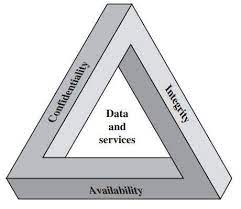
\includegraphics[scale=0.7]{Figures/cia_traid}
\caption[CIA гурвалжин]{CIA гурвалжин}
\label{fig:Electron}
\end{figure}

Шифрлэлт ерөнхийд нь гурав ангилна.
\begin{itemize}
    \item \textbf{Тэгш хэмт шифрлэлт (symmetric):}
    \item \textbf{Тэгш бус шифрлэлт (asymmetric):}
    \item \textbf{Хаш (Hash)}
\end{itemize}

Нууцлаг байдлыг хангахад
\begin{itemize}
    \item Тэгш хэмт шифрлэлт (symmetric)
    \item Тэгш бус шифрлэлт (asymmetric)
    \item Хаш (Hash)
\end{itemize}

Бүрэн бүтэн байдалыг хангахад ашиглана.
\begin{itemize}
    \item Хаш (Hash)
    \item Мессежийн баталгаажуулалтын код (MACs)
    \item Тоон гарын үсэг (Digital Signatures)
\end{itemize}

%-------------------------------------------------------------------------------
%	SECTION 2
%-------------------------------------------------------------------------------

\section{Орчин үеийн ширфлэлтийн схемүүд}

Identity-based encryption (IBE): This is a type of public key encryption that allows users to encrypt and decrypt data using their identities instead of public keys. IBE can be used for secure data sharing in scenarios where users are known by their identities.

Attribute-based encryption (ABE): This is a type of encryption that allows access to data based on predefined attributes, such as age, job title, or organizational role. ABE can be used for fine-grained access control to data, and can be used in scenarios where access is granted based on certain attributes.

Homomorphic encryption (HE): This is a type of encryption that allows computations to be performed on encrypted data without first decrypting it. HE can be used for secure data processing in scenarios where data needs to be kept confidential while still allowing for computation.

Secure multiparty computation (MPC): This is a cryptographic technique that allows multiple parties to jointly compute a function over their private inputs without revealing their inputs to each other. MPC can be used for secure data processing in scenarios where data needs to be kept confidential and multiple parties need to collaborate.

%-------------------------------------------------------------------------------
%	SECTION 3
%-------------------------------------------------------------------------------

\section{Proxy Re-Encryption схем}

Прокси дахин шифрлэлт нь нийтийн түлхүүрээр шифрлсэн өгөгдөлийг дахин ширфлэж өөр хувийн түлхүүрээр тайлах боломжийг олгодог.

Давуу талууд:
Гурав дахь сервер гэх мэт өгөгдлийг байршуулах боломжтой.

Сул талууд:

Үндсэн хоёр төрөлтэй.

Unidirectional PRE: Зөвхөн нэг талдаа дахин шифрлэх боломжтой.

Bidirectional PRE: 2 талдаа дахин шифрлэх боломжтой.

Some features of PRE schemes include:

Delegation: PRE allows data owners to delegate access to their data to third-party entities, without giving them complete access to the data.

Access control: PRE allows data owners to control who can access their data and under what circumstances, even after the data has been shared.

Efficiency: PRE can be more efficient than traditional re-encryption techniques, as it does not require the data to be decrypted and re-encrypted.

Security: PRE provides a high level of security, as the proxy does not have access to the data itself and can only transform the encrypted dat

%-------------------------------------------------------------------------------
%	SECTION 4
%-------------------------------------------------------------------------------

\section{Бүлгийн Дүгнэлт}